\label{sec:classification}
\section{Identification of jobs with environmental functions}

Because many of the job offers provided by X28 are not actually environmentally related, a classifier is developed to predict whether or not a given job is relevant to the research question. The aim is to build a classifier that can split the the jobs into environmentally related and non-environmentally related offers. Neural networks are machine learning algorithms named and modeled after the way neurons in the human brain deciphers complex information. These neurons allow the brain to to recognize, categorize, or process certain occurrences in the world around us. Artificial neural networks are designed after this biological function. A simple example of a basic neural network is shown in Fig.~\ref{fig:basicNN}, and is made up of an input layer, one or more hidden layers, and an output layer. 

\begin{figure}[htbp]
  \centering
    \includegraphics[width=0.7\textwidth]{figures/BasicNN.pdf}
    \caption{
    An illustration of a simple neural network with one hidden layer.
    }
\label{fig:basicNN}
\end{figure}



Each neuron, or node of the network, takes numerical input, applies an operation on the input, and outputs a modified value to each neuron to which it is connected. For each connection in the network, the inputs are multiplied by a different numeric value, which constitute the \emph{weights} of the network. The multiplied values are then input to the activation function of the neuron, which provides a non-linear operation for the data, a key aspect that allows the neural network to form a very flexible function capable of predicting complex properties. The activation function effectively determines which neurons are ``activated,'' that is, are above a certain numerical threshold, and therefore pass information to the next layer of neurons as a numerical output. The weights can take different values and are optimized during the training of the model. Several different activation functions can be used, such as the sigmoid or Relu functions. These functions help decide the output of the neurons. 

An simple illustrative example showing how the inputs are transformed in a single node is shown in Fig.~\ref{fig:simplenetwork}. Neural networks can take on a variety of architectures with varying numbers of layers of neurons and different activation functions. The layers can be connected in different ways. In the models utilized for this research, dense, or fully connected layers are used. This means that all the neurons from one layer are connected to all the neurons in the following layer. This is illustrated in Fig.~\ref{fig:fullyconnected}. In classification tasks, the final layer of the network produces numerical values which at different thresholds allow the the model to make different predictions. 

\begin{figure}[htbp]
  \centering
    \includegraphics[width=0.5\textwidth]{figures/SimpleNeuron.pdf}
    \caption{
    An illustrative example of a simple artificial neuron.
    }
\label{fig:simpleneuron}
\end{figure}



\begin{figure}[htbp]
  \centering
    \includegraphics[width=0.3\textwidth]{figures/FullyConnected.pdf}
    \caption{
    An illustrative example of fully connected layers in a neural network.
    }
\label{fig:fullyconnected}
\end{figure}

A neural network model is chosen for the classification of environmentally related and non-environmentally related jobs because of their ability to handle complex, multidimensional data sets, such as human language. They provide the ability to group or classify unlabeled data through unsupervised learning. Human language contains many nuances and complex vocabulary structures, and neural networks have the ability to deal with abstraction.  

Two neural network architectures are developed and compared. The first architecture is the simpler of the two and is shown in Fig.~\ref{fig:simplenetwork}. In this architecture, there is only one input layer, which is the  cleaned and English-translated text of the job offers. The Keras layer encodes the text using the Universal Sentence Encoder~\cite{DBLP:journals/corr/abs-1803-11175}, described further in Section~\ref{sec:activites} using the dedicated Keras interface provided by TensorFlow Hub, and produces an output of a 512-dimensional vector for each sentence. The output of the Keras layer is then fed into the first dense, or fully connected, layer. This means that each input is fed to each individual node, or neuron, of the neural network. These neurons have their own set of weights that are optimized during network training via backpropagation, which when trained helps the neural network learn which features have a more weighted affect on the model's output. The output of the first dense layer therefore are 256 numbers that are obtained by a weighted combination of the vectors and the neurons. All dense layers use the Relu activation function. This simple function, shown in Equation~\ref{eq:relu}, takes a value of 0 for negative inputs, and the input value if the input is positive. 

\begin{equation}
f(x) = \max(0, x)
\label{eq:relu}
\end{equation}

The second dense layer takes in the input of the 256 numbers from the first dense layer, and uses 32 neurons to compute the output, again using a weighted linear combination and the Relu function. Finally, the third dense layer takes in the 32 numbers as an input, and a single node outputs either a 0 or 1 value, using a sigmoid activation function, shown in Equation~\ref{eq:sigmoid}.

\begin{equation}
f(x) = \frac{1}{1+e^{-x}}
\label{eq:sigmoid}
\end{equation}

A value of 0 means that a job offer is classified a non-environmental, and a value of 1 means the job offer is classified as environmental.


\begin{figure}[htbp]
  \centering
    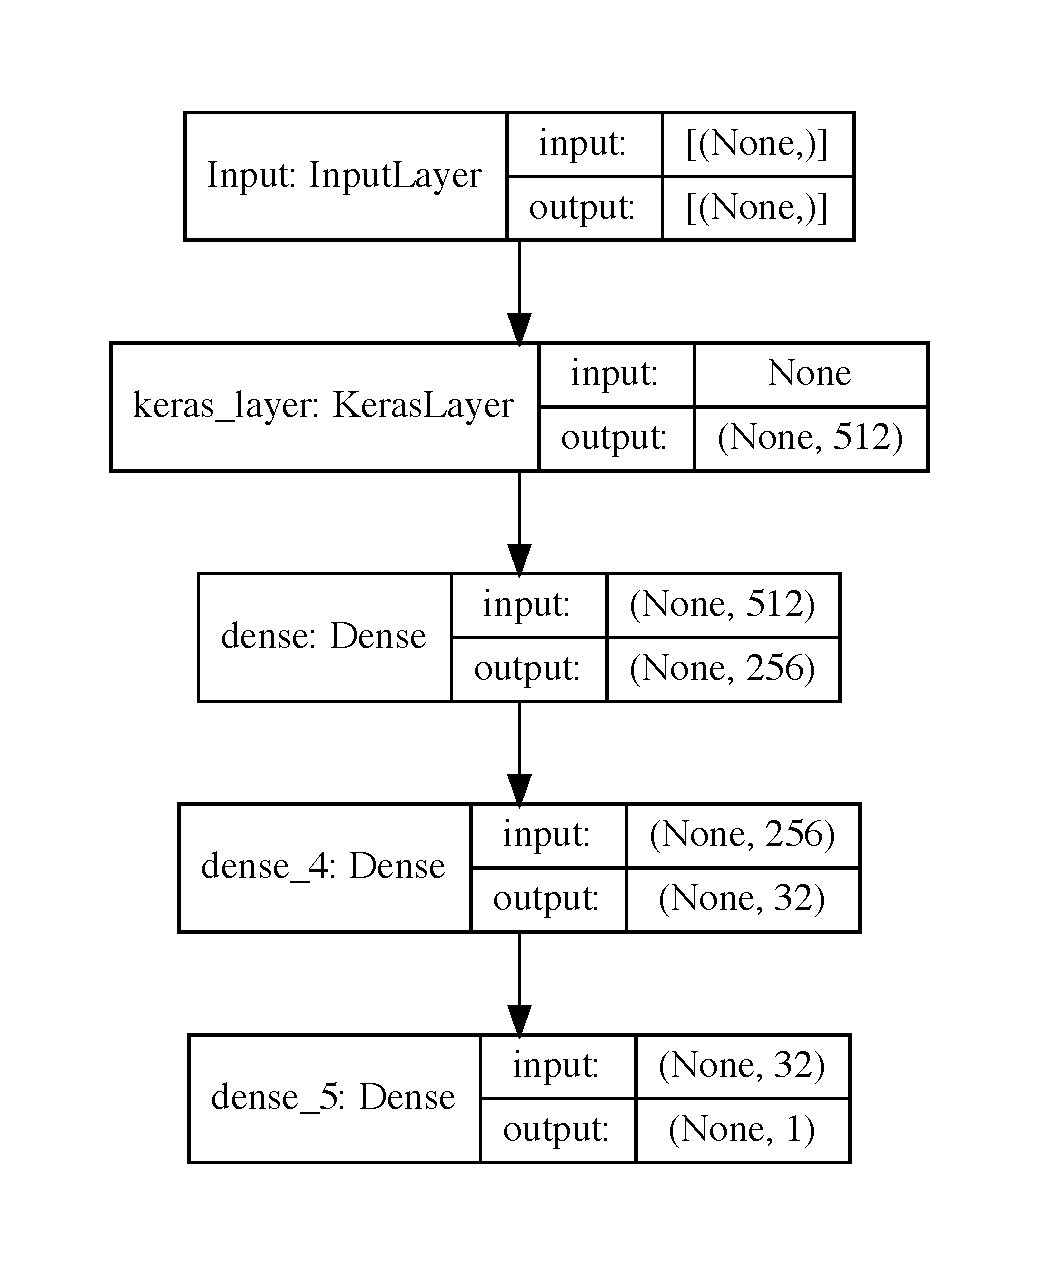
\includegraphics[width=0.7\textwidth]{figures/NeuralNetArch_OnlySentences.pdf}
    \caption[The simpler neural network architecture used in the classification of environmental and non-environmental job offers]{
    The simpler neural network architecture used in the classification of environmental and non-environmental job offers. In this architecture, only the encoded text is used as input.
    }
\label{fig:simplenetwork}
\end{figure}


The second architecture is shown in Fig.~\ref{fig:fullnetwork}. The input layer on the top left refers to the cleaned and translated text of the job offers. The architecture of the network for the layers connected to this input is very similar to the architecture described in Fig~\ref{fig:simplenetwork}. However, this neural network utilizes a separate input layer, labeled input\_1 and shown to the top right of Fig.~\ref{fig:fullnetwork}. This layer takes in a number of other categorical and numeric features of the data. These variables are the number of sentences normalized, the number of characters normalized, the company size represented as a categorical variable, and the canton size represented as a categorical variable. 

\begin{figure}[htbp]
  \centering
    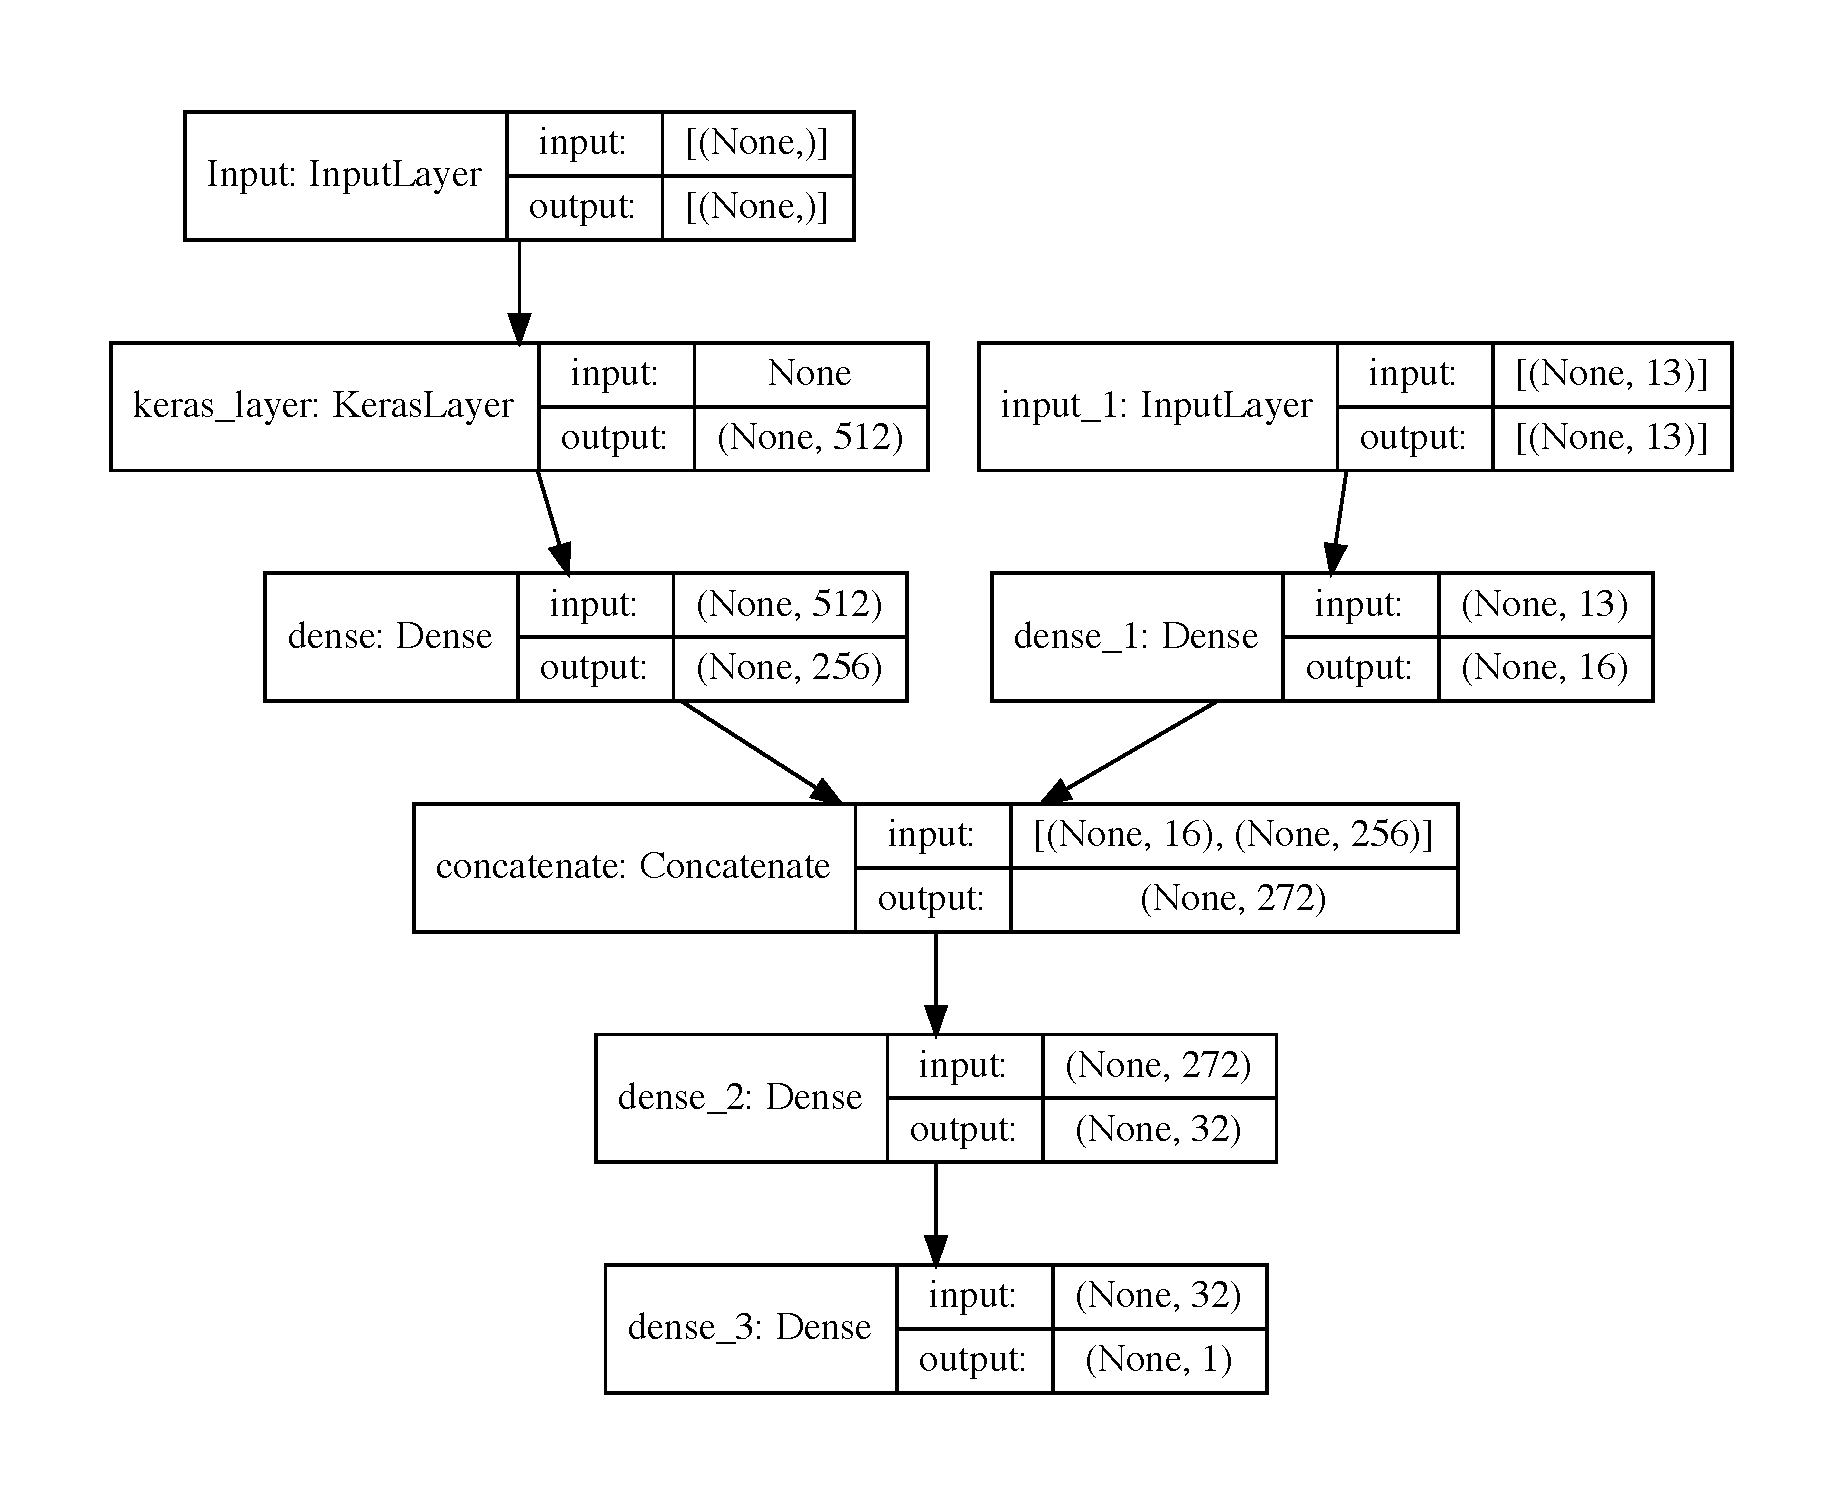
\includegraphics[width=0.7\textwidth]{figures/NeuralNetArch_AllInputs.pdf}
    \caption[The more complex neural network architecture used in the classification of environmental and non-environmental job offers]{
    	The more complex neural network architecture used in the classification of environmental and non-environmental job offers. This architecture takes in the number of sentences in the job offer, the number of characters in the job offer, the size of the company offering the job, and the canton the job is advertised in.
    	}
\label{fig:fullnetwork}
\end{figure}

The number of sentences and the number of characters are normalized by the mean and standard deviation such that the mean and standard deviation are 1. This is done because normalized data is preferred by the neural network, because a large spread in magnitude of input values tends to lead to larger weights in the network and less stable training. The categorical variables are represented by dummy variables rather than by single variables that takes on multiple values. These dummy variables can only take on values of 0 (false) or 1 (true), and as such, they serve the purpose of distinguishing the categories as distinct. Because it is also possible for a company size to be 'uncategorized', the company size variable is represented by four dummy variables. It is not possible for two or more of the dummy variables representing the company size to take a value of 1; however, it is possible for all to be 0, indicating an uncategorized company. For the job's canton, 7 dummy variables indicate whether or not the job takes place in the given canton. It is possible for jobs to cover multiple cantons, or for the job to be in another canton than the 7 most common, which corresponds to a configuration of all dummy variables zero.

Including all the dummy variables, the network considers 13 numeric inputs. The numeric inputs are fed to a dense layer with 16 nodes, which combine the inputs and utilize a Relu activation function, again shown in Equation~\ref{eq:relu}. The 16 numeric outputs of the 16 neurons are concatenated with the 256 numeric results from the dense layer connected to the inputs of the converted sentences to form a concatenated layer of 272 values, as shown inn the center of the figure. These outputs are then fed to a dense layer of 32 neurons before being compressed into a single output layer. The output layer uses a sigmoid activation function, again shown in Equation~\ref{eq:sigmoid}, in  order to compress all inputs to a single number between 0 and 1. The prediction of the network is derived from this result. Values less than 0.5 are then consider false, or not environmentally related in nature, and values greater than 0.5 are taken as environmentally related. 

The use of the Universal Sentence Encoder embeddings allows the model to benefit from the huge training data set used by Google to develop the pre-trained model. However, this data set is not specific to the environment activities categorization task. Through transfer learning, the neural network sculpts the pre-trained inputs towards the task at hand. This approach allows the training to be performant with a much smaller input data set than would be needed to train a NLP model from scratch only using labeled job offers. This approach is essential to this task, because the labeled data set must be tediously constructed by hand, and is therefore of very limited size.

Both models are trained and optimized using the subset of 536 job offers which are labeled as environmentally related or not. Of the 536, 304 are environmentally related, and 237 are not. In order to build a more balanced data set, only two-thirds of the non-environmentally related jobs are used in the training set. A total of 180 job offers are used for the test data set. There are several parameters and hyperparameters that can be optimized within neural network models. These include the learning rate, the number of layers, the batch size, the number of epochs, and the learning rate decay. The learning rate is generally regarded as one of the most important parameters to tune, since it can result in larger performance increases while not adding great amounts of computing time. The number of epochs is also a commonly tuned parameter, with more epochs often improving accuracy, but this usually comes at a higher time cost. Therefore, the learning rate methods and the number of epochs are manipulated in the more complex neural network model in order to improve model accuracy. 

Confusion matrices are made to visualize the performances of the neural network models. A confusion matrix is a table that displays four different combinations of predicted and actual values. The top left quadrant of the confusion matrix displays the number of false predictions which are indeed false. These are called true negative (TN) predictions. The top right quadrant displays the number of true predictions which were actually false. These are called false positive (FP) predictions, or Type I error. The bottom left quadrant displays the number of false predictions which were actually true. These are called false negative (FN) predictions, or Type II error. Finally, the bottom right quadrant displays the number of true predictions which are indeed true. These are called true positive predictions (TP). Using these tallies, it is possible to calculate different metrics to evaluate the models. The recall of the model describes the fraction of relevant instances that are retrieved. The recall equation is shown in Equation~\ref{eq:recall}.

\begin{equation}
\text{Recall} = \frac{TP}{TP + FN}
\label{eq:recall}
\end{equation}

The precision of the model is the fraction of relevant instances among the retrieved instances. The precision equation is shown in Equation~\ref{eq:precision}.

\begin{equation}
\text{Precision} = \frac{TP}{TP + FP}
\label{eq:precision}
\end{equation}

It is ideal to have precision and recall as high as possible, but often they have an inverse relationship. That is why the F-measure is often used as a more holistic metric that combines the precision and recall together. The F-measure equation is shown in Equation~\ref{eq:F}. The F-measure then can be used to identify the best-performing neural network model. 

\begin{equation}
F_{1} = \frac{2 \times \text{Recall} \times \text{Precision}}{\text{Recall} + \text{Precision}}
\label{eq:F}
\end{equation}

The two neural network architectures are compared, with the F-measure taken as the metric of interest to define the optimal model. The hyperparameters of the network, that is, the parameters of the model that are not fixed but are determined by the problem at hand, including the learning rate, number of epochs and batch size, are optimized to achieve the best performance with the labeled data set. The results and the optimal parameters are further discussed in Chapter~\ref{chap:Results}, Section~\ref{sec:greenresults}.

Why don't you add the total number of weights (can get this from model.summary() in Keras)?

You should say what batch size and number of epochs you use. Then you should spend a little bit of effort trying to optimize the network to get the final ac ]] from the two.




